\documentclass{article}
\usepackage[margin={2cm,2cm}]{geometry}
\usepackage{multicol}
\usepackage{graphicx}

\begin{document}

\title{Large Scale Network Analytics Using Distributed Servers}
\author{Ryan McGrath}
\maketitle

\begin{abstract}

  Analysis of network traffic is necessary for network management and defense. However, analysis of large network packet captures is difficult due to proportional memory and processing requirements for the quantity of network data. Wireshark, a popular packet analyzer, can have a memory requirement of multiple times its size. This makes it difficult for a single host to analyze multi-gigabyte capture files.  This paper presents a system to divide, distribute, query, and efficently load balace analytics for large packet captures using a distributed system of lightweight servers. This enables network analysis techniques for small network captures to scale to gigabyte-sized captures.


\end{abstract}


\begin{multicols}{2}
  
\section*{Introduction} % \section* would create section without section
                       % number.


Packet analyzers enable analysts to examine individual packets.  An analyzer decodes the structure of network protocols encapsulated in the packet and can have a filtering syntax to preform queries.  These queries can uncover misconfigured networks, misbehaving users, or even network intrusions. The overwhelming volume of normal traffic makes it difficult to discover limited, infrequent malicious events. This difficulty is compounded as the dataset scales. Packet analyzers have a high memory requirement \cite{wireshark} because they reassemble packet sessions and model layers of network protocols.  Other packet analysis tools, such as tcpdump and ngrep, do not create dependencies between packets and filter selected packets in a single pass. While these tools have a lower resource requirement, analyzing large datasets can still be time-consuming. 

This paper presents a system to enable packet analyzers to analyze large datasets by using a distributed system. The system distributes a portion of the network data to each server, issues commands, collects the results, and balances the amount of data on each server to optimize repeated queries. The central server issues commands over SSH and transfers files using rsync to processing servers. The load balancing algorithm adapts for differences in server resource capabilities and data by redistributing the chunks of data each server processes. This improves repeated queries against the same dataset. This system enables a cluster of heterogeneous servers to rapidly divide a large network capture and run queries in parallel. 

The syntax of the queries are tshark, tcpdump, or ngrep commands. These tools have a robust filtering syntax that is well-known. Building upon widely used open-source tools enables reuse of optimized packet processing libraries and support for hundreds of protocols. This avoids the complication of translating network data to fit a specific query syntax.  

The system is designed for a variety of use cases. One use case is to develop the query on a subset of the packet capture on a single machine and use the system to run the query against the full dataset.  Another use case is to filter a large dataset to produce output for a consuming analytic. The output can be sent using unix pipes to tools such as sort, uniq, or count. 

The system could be implemented using a commercial cloud provider to add additional servers until the desired performance is reached. Alternatively, the servers could be laptops that are transported to a client site to function as a tool to support network incident response.

\section*{Related Work}

Several approaches have been developed to analyze traffic and monitor large scale networks. One approach, commonly called netflow, is to reduce the size of the captured network data by storing the metadata. This metadata, such as listing source and destination IP addresses, can be analyzed for anomalies.  This approach requires prior knowledge of what is necessary to capture, and discards most network content. Intrusion Detection Systems (IDS), such as Snort, take a different approach by scanning traffic for pre-defined signatures. The open source Bro network security monitoring system combines a netflow approach with IDS-like functionality.  Other efforts, such as pcap2sql, translate relevant network events into a database. These approaches enable queries on network data, but are limited by the requirement to know exactly what to extract from network traffic. 

Other efforts have focused specifically on analyzing large network captures. Network traffic has limited dependencies and can be split into parallel workloads for servers to analyze individually.  Techniques from Lee and Lee \cite{lee2013}, and Nagele \cite{ripecc2011} both use a Hadoop-based approach to distribute work among a number of servers.  Lee and Lee's system ingests netflow data and utilizes custom analytics for network statistics while Nagele has developed a distributed DNS-based analytic and supports SQL-like queries against the captured data.  Both systems require the overhead and complexity of a Hadoop system, translation of the network data to an optimized format, and are tailored for specific analytic uses.  Packetpig is another effort that works on large network captures and utilizes Hadoop to run Apache Pig queries against captured traffic. 

\section*{Methods and Design}

The three primary components of the system are the distribute, command function, and load balancing functions. The distribute function splits the packet capture data among the processing servers. The command function executes the packet analysis query on each server.  The load balancing function transfers data between nodes to optimize another query against the same dataset.

In the distribute function,  the central node splits the network packet captures into chunks which are distributed equally among the processing nodes.  A capture is split into 25 megabyte (MB) chunks. The chunk size is important because the memory requirment can be multiple of the files size on disk. This chunk size was selected because it preformed well with the limited resourced Virtual Machines (VM) that were used in development.  Before files are distributed, the central server queries each processing server for files have already been distributed. Then, only files which have changed are transfered.  This allows for efficient repeated queries of a dataset that continues to grow.  All remote communications utilizes SSH public-private key pairs to provide authentication and a secure channel.  The distribution is made using the rsync program running over SSH, and compressed.  Chunks are distributed in a round-robin method among the processing servers so if a single portion of the capture is more complex to analyze, there is a chance that it is distributed equally among the processing servers.      

In the command function, the central node executes a tshark, ngrep, or tcpdump command on each processing node against the distributed data. The central server uses the user-provided command to construct a bash for-loop that runs on each processing server. An SSH session is established with each processing server concurrently using the python threading library.  Each processing node executes the command against their local allotment of the network data and returns the output and its execution time to the central server. The data is collected from each thread in a thread-safe data structure and sent to standard output in order of completion.

The load balancing algorithm minimizes the disparity in completion times between nodes by orchastrating the transfer of data chunks between poorly performing servers and highly preforming servers. This lowers the overall task completion time.  The central node records the task completion time for each node.  If the completion time of a processing server is above a user-specified percentage threshold of the average completion time of all nodes, the central node marks it as a slow server. If the processing server is below the threshold, it is marked as a fast server.  The central node calculates a number of randomly selected files to transfer from the slow to fast servers to move the slower server completion time closer to the average. The number of transfered files is determined by calculating the average time processing each file on the slower node.  Then, the slow server's completion time is subtracted from the average completion time all nodes and divided by the server's average time per file. This ceiling of this result is the number of files to tranfer. The slowest overall server randomly selected files and transfers them to the fastest server.  The process is repeated with the second slowest and fastest servers, and so on, until there is not a pair of servers that performed outside of the threshold.  Transferring files in proportion to the difference from the average completion time moves slower servers quickly towards the average completion time of all nodes.  This accomplishes two goals, utilizing more of high resourced servers in a hetrogenous cluster and leveling the distribution of sought-after network data throughout the cluster.  An example of sought-after data would be if a queries targets a specific network device, and traffic from this device only occurs in chunks of the network capture concentrated on a single processing server which will slow its execution time.  Eventually, the load balancing algorithm will distribute these sought-after chunks among a greater number of nodes. 

\section*{Evaluation} 


The objective is to determine the degree of parallelism exhibited by this system and specifically to evaluate the efficentcy of the load balancing algorithm. The query extracts all DNS queries out of a 695 MB packet capture and is evaluated by varying the number of nodes, and the effectiveness of the load balancing algortihm.  The dataset is split into 26 chunks, however the time to process each chunk is not equal.  Since the query only considers DNS traffic the amount of DNS traffic is the crtical factor for execution time as other traffic can be discarded quickly.  Figure () shows the relevant statistics of the dataset which was determined by counting the DNS entries per chunk.  There is a large standard deviation between chunks that can cause unequal running times on each processing server.qD

\begin{tabular}{llr}
\hline
\multicolumn{2}{c}{Dataset Statistics} \\
\cline{1-2}
Size & 695 MB \\
Records & 27 \\
Sum & 17604 \\
Average & 653 \\ 
Standard Deviation & 526.83 \\
Median & 419 \\
Max & 2393 \\
Min & 80 \\
\hline
\end{tabular}


The tests were conducted using Virtual Machines (VM) allocated 512 MB of RAM and a single core processor. The ''large'' VMs were alocated 1GB of RAM.  All VMs are hosted on an 8 GB RAM, quad-core Apple iMac. Since resources need to be reserved for the host operating sytem, a limited number of VMs can run at once.  Tests with more VMs running can be affected by competition for processor time, disk access, background activity of the host, and the overhead of running the VMs.  This is a limitation to evaluating this system as an ideal evaluation would use a large number of dedicated servers to test the system at scale.

Figure () shows the task completion times for ten repeated queries with different numbers of processing servers.  The completion time decreases as the number of nodes increases, until more than four servers are used. The load balancing algoritm contributes to a decreased completion time until after the four server configuration.  At this point, for both approaches, the overhead outpaces any gains from adding more nodes to divide the work.  This limit could be the result of of running more than four VMs affected the running time.  Since the host machine has a quad core processor, running more than four VMs could contention on CPU core and increases the completion time.

\noindent\makebox[\linewidth]{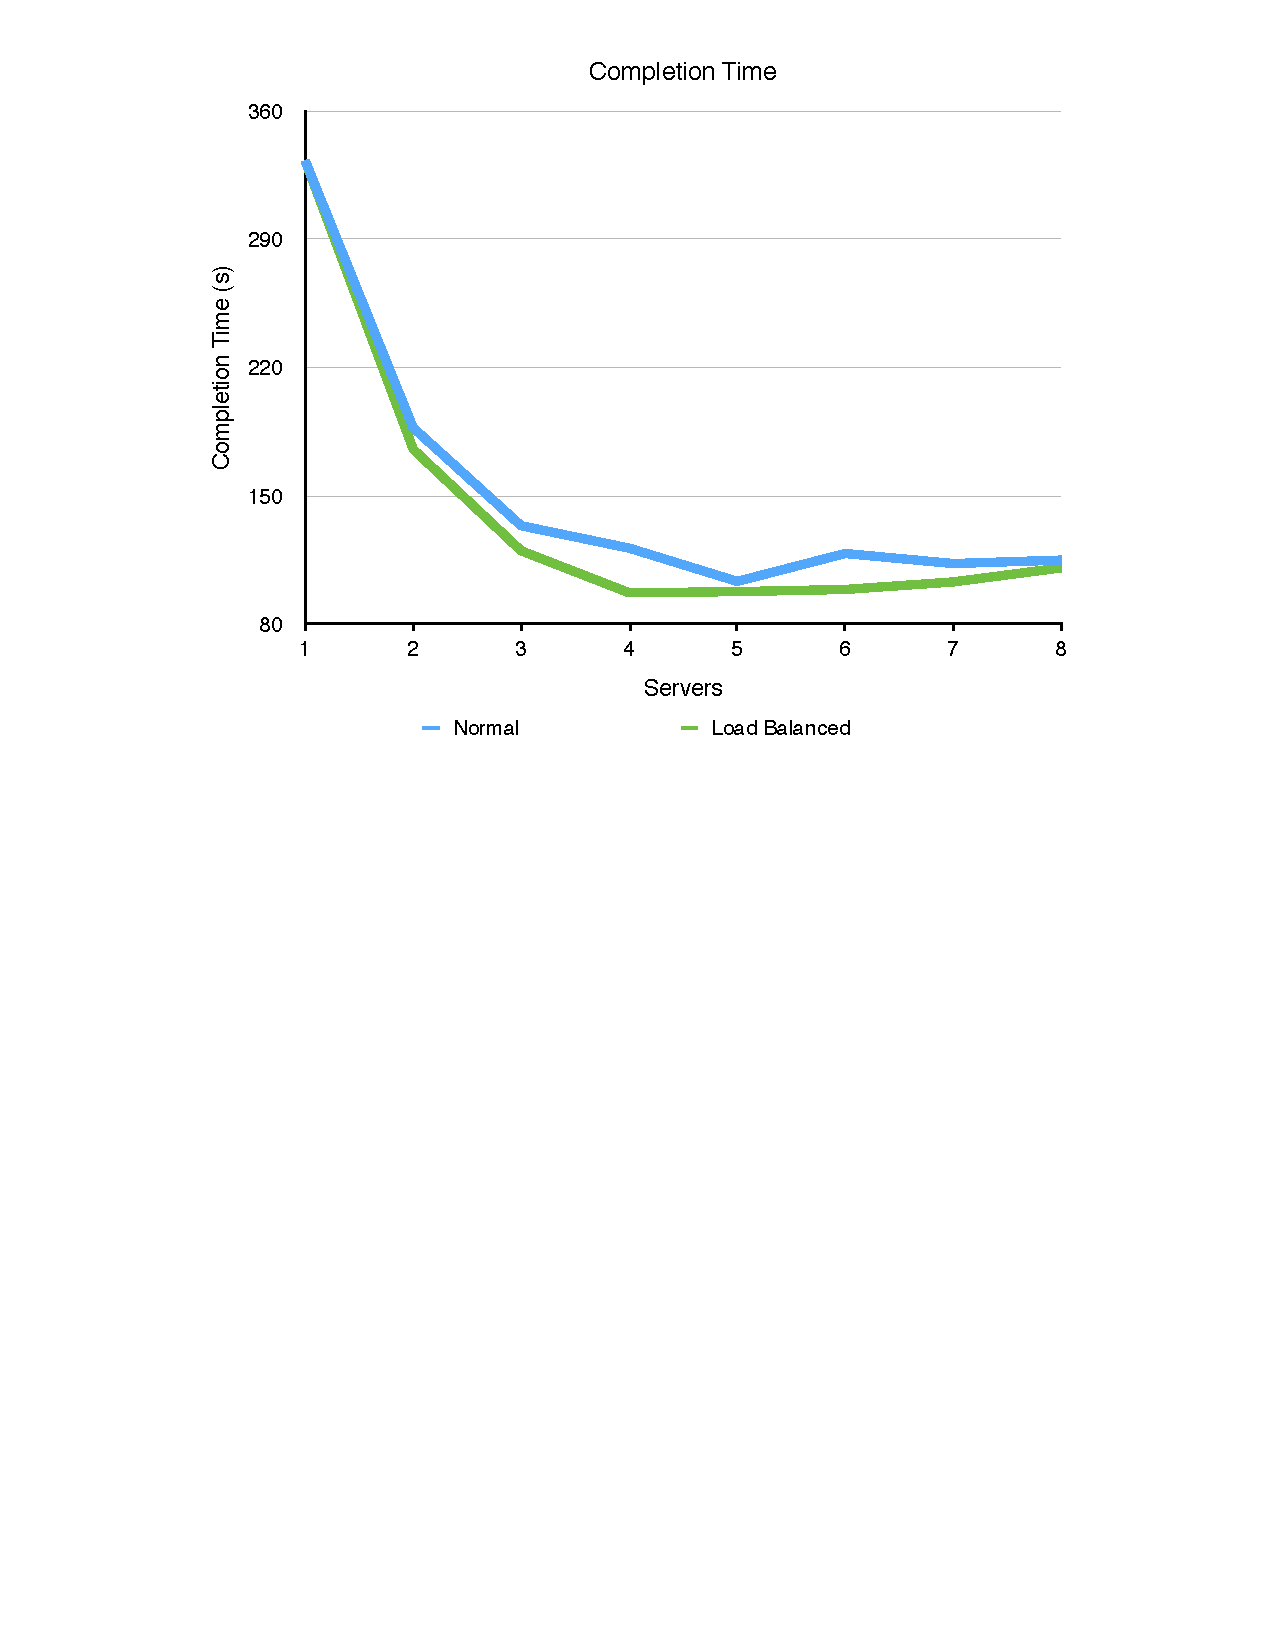
\includegraphics[width=\linewidth]{CompletionTime.pdf}}

Examining the performance of the four server cluster, figure () show the differnce in completion time when using the load balancing technique.  The green, broken line, shows the performance of four servers with randomly distributed chunks. The blue, solid line, shows the performance when the load balancing algorithm is applied after one query with the random distribution of chunks.  After the first query there is a marked decrease in completinon time which generally persists for repeated queries.  The completion time with load balancing is 17.1 percent less than the average completion time without load balancing.  However, the algorithm can make a data tranfer that adversaly effects the running time because only the average cost per chunk is calculated rather than knowing the actual cost per chunk. This means an ineffcent transfer can be made, but the algorithm will self correct on the next iteration attempting to reach the threshold. Once achieved, the algorithm stops transfers until the threshold is breached. One theoritical negative situation would be if a chunk wasoverwhelmingly computationally expensive that after each query, the algorithm would continually moving this chunk from server to servers without reaching the desired threshold.  While this situation was not encountered during testing, a smaller chunk size would split this computationally expensive data and be effectively distributed across servers by the load balancing algortihm. 

\noindent\makebox[\linewidth]{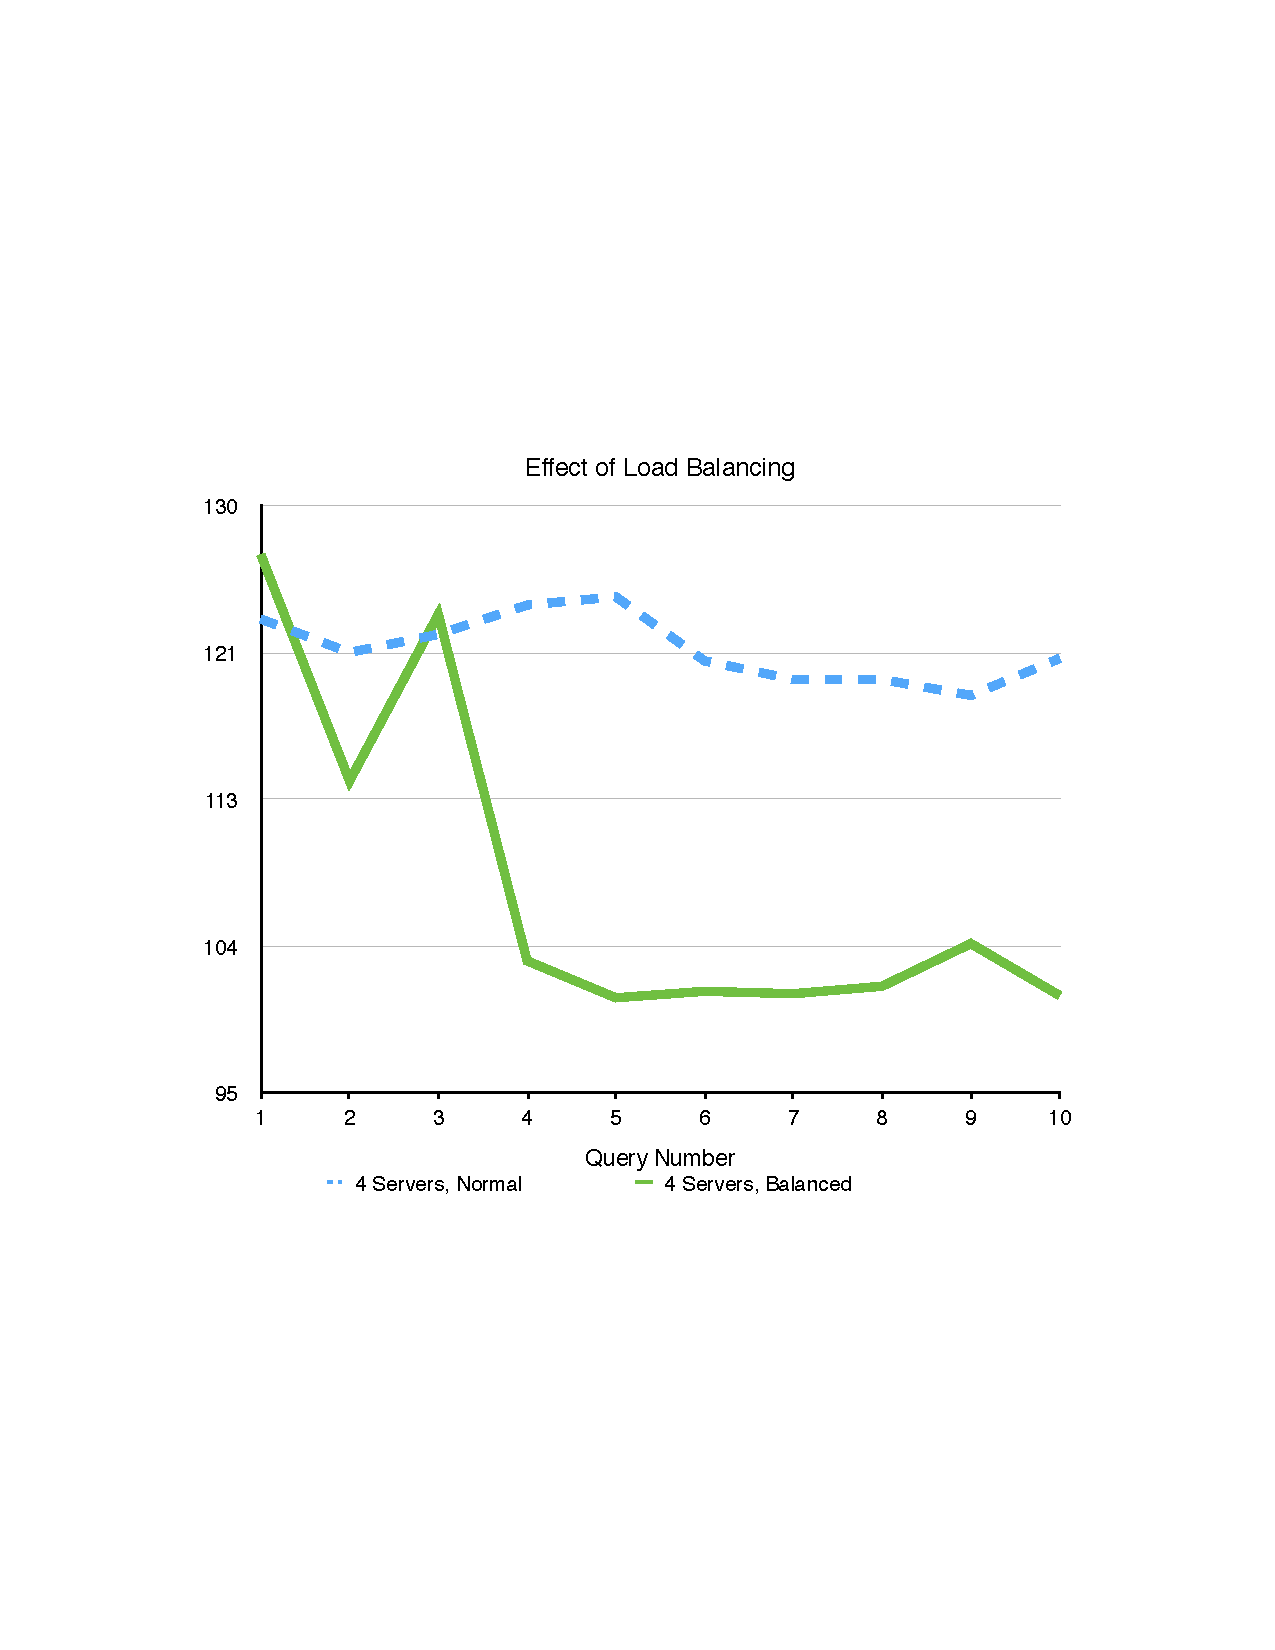
\includegraphics[width=\linewidth]{LoadBalancingEffect.pdf}}

Another measurement of the load balancing algorithm is seen in the figure (), the standard deviation of the individual server completion times when using four servers and eight servers.  Without load balancing, there is a realtively constant standard deviation.  The effectivness of the load balancing is seen in the reduction of the standard deviation after the first query.  This reduction results in a lower overall task completion time which is seen in Fig ().

\noindent\makebox[\linewidth]{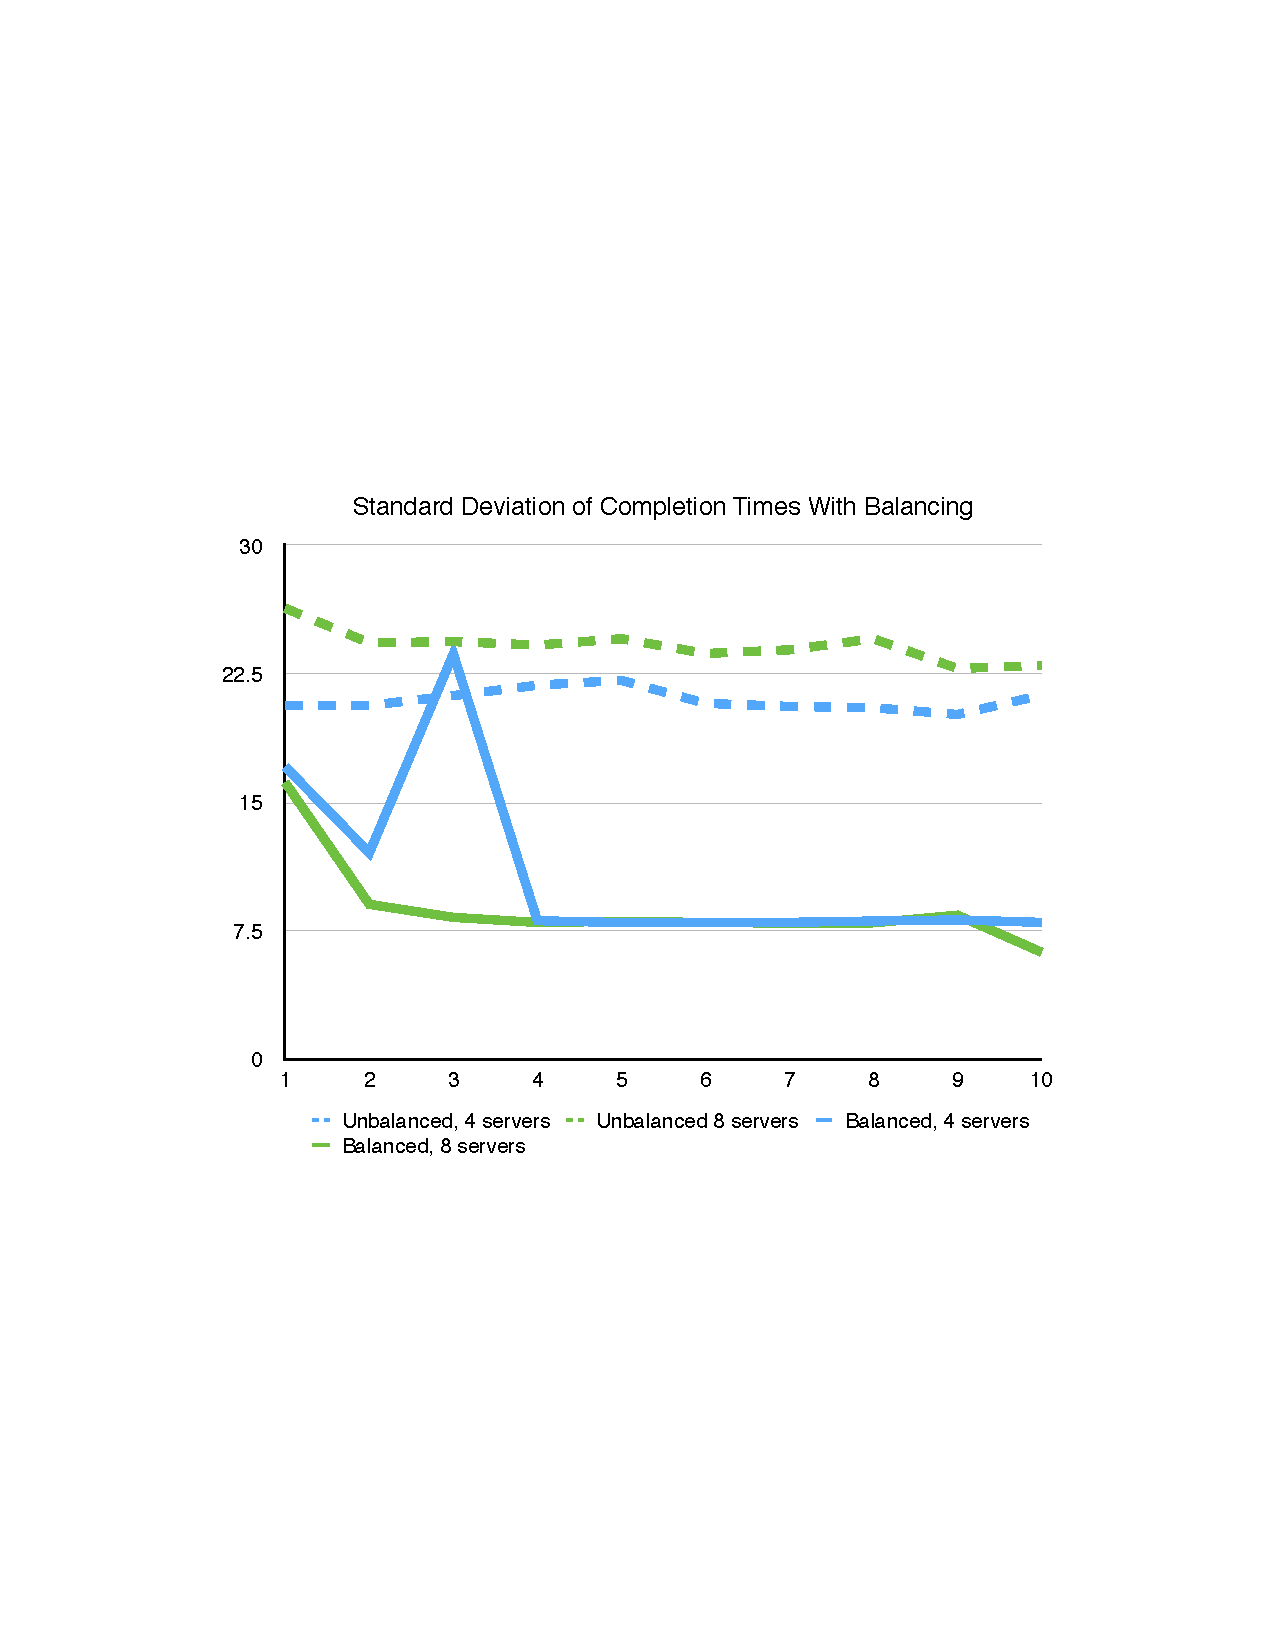
\includegraphics[width=\linewidth]{StandardDeviation.pdf}}

When adding addtional processing capacity to a distributed system, the best performance is called linear speedup.  This means that as the number of processing servers is doubled, the speedup would double. Speedup is defined as the execution time for a single server to complete the task divided by the execution time for the multiple server configuration.  For this system there is a less than linear speedup, and loss of improved perfomance after four nodes.  Figure () shows a table of the speedup and efficiency results.  Efficentcy is a metric that represents the utiliztion percentage of each server by diving the speedup factor by the number of servers.  An efficentcy of 1 would indicate perfect speedup.

\begin{tabular}{llr}
\multicolumn{3}{c}{} \\
\cline{1-3}
Servers    & Speedup & Efficiency  \\
\hline
1     &  1  & 1   \\
2     &   1.77  & .88  \\
4     &   2.73  & .68 \\
4 (balance) & 2.97 & .74     \\
8 &  2.89   & .36  \\
8 (balance) & 2.93 & .36      \\
\hline
\end{tabular}

Figure () shows the efficentcy per node as the number of servers increases.  The blue, broken line shows the efficiency of the system with a random distribution of data to the servers, while the green, solid line represents the increased effeciency when using the load balancing algorithm.  The load balancing algorithm increases the efficentcy of the system over a random distribution, but again, this approach is ineffective past the limit of four servers.

\noindent\makebox[\linewidth]{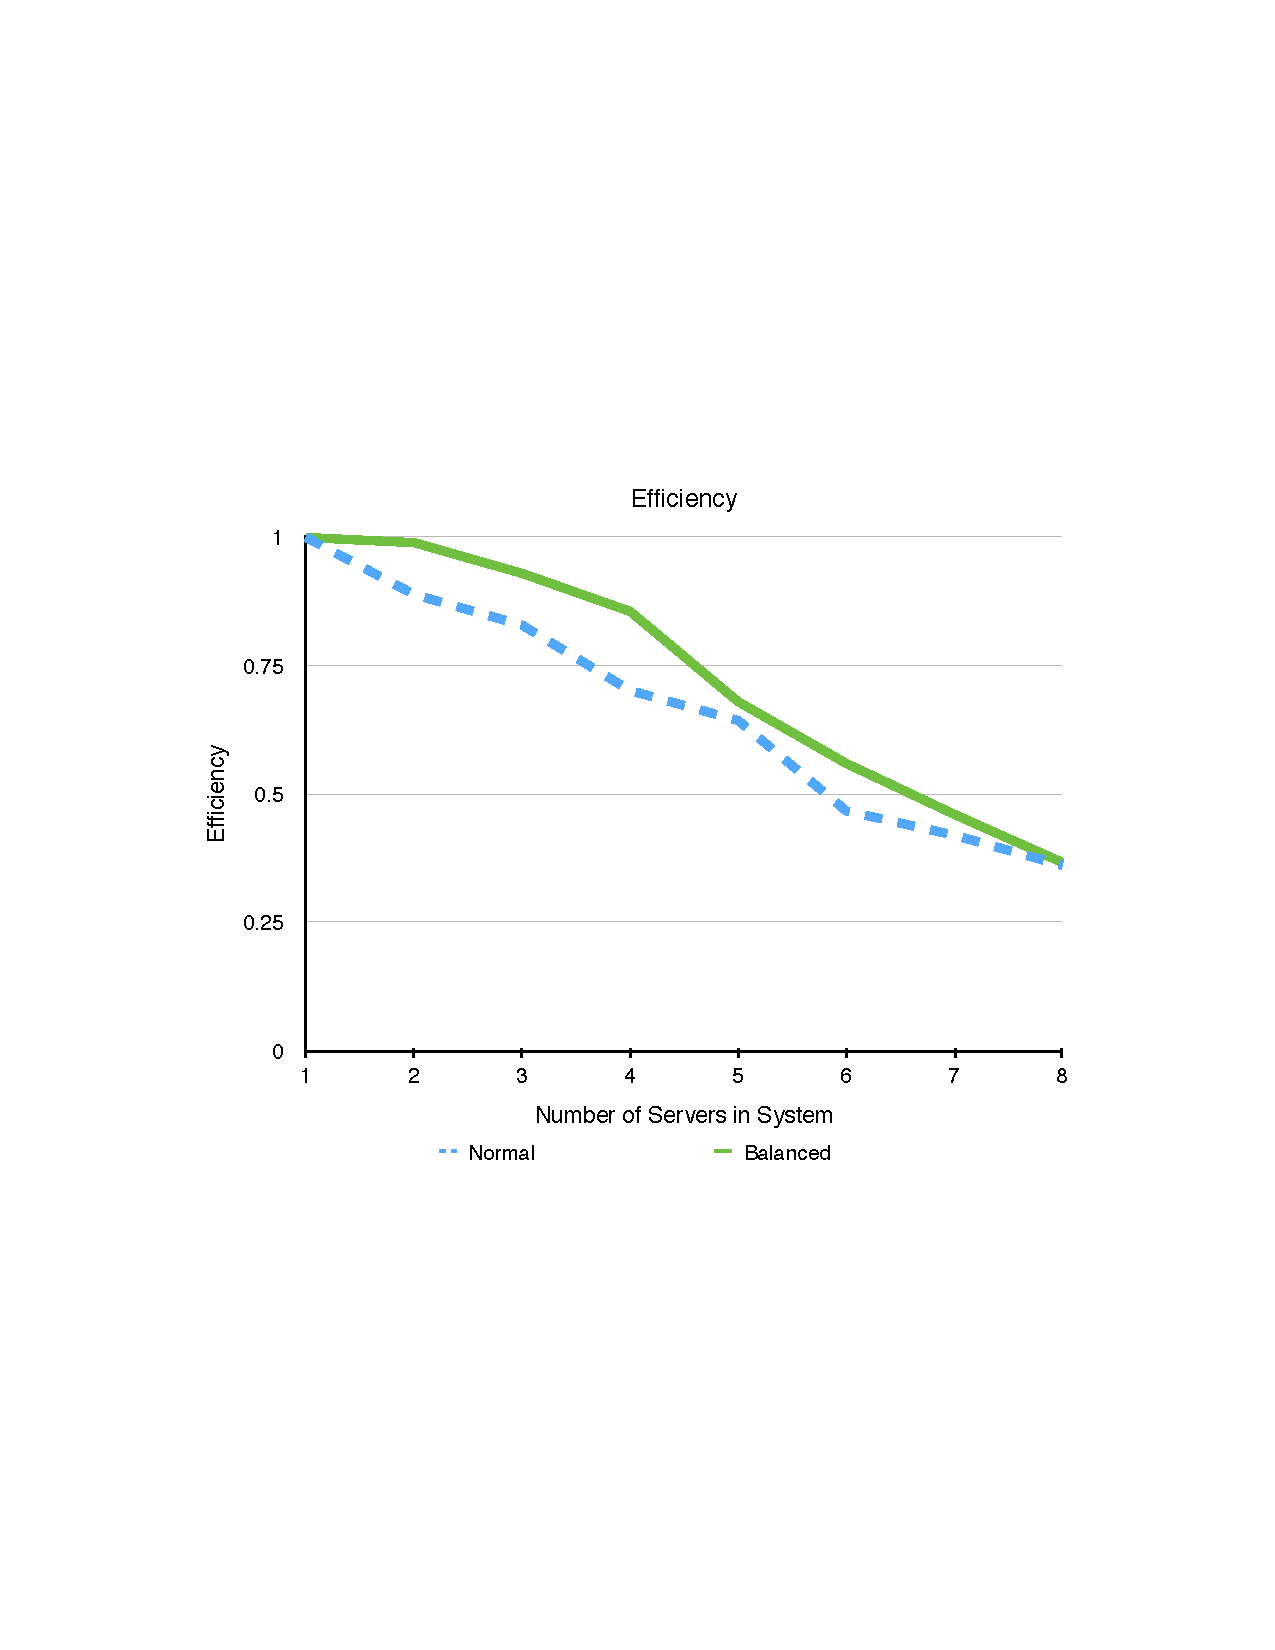
\includegraphics[width=\linewidth]{Efficiency.pdf}}


In spite of the testing hardware limitations these results provide encouragement that the parallization and load balancing techniques would scale with dedicated hardware and larger datasets.


%Talk about modifying the threshold percentage time, and using ''big'' nodes???

There are limitations of this system that were not addressed in this effort.  As the system scales, the central node could become overwhelmed with network traffic as it becomes a hotspot with all communicaiton leaving and returning to it. One extension could have nodes assisting with data transfer in a peer-to-peer arrangement instead all transfers originating with the central node.  Another improvement would be to accomidate node failures. One approach would be to track the files that were on the failed node and to re-distributed them to a functioning node.  Another issue is the possibility that the central node could be overwhelmed by a large amount of results. The result of a query could overflow the bounded buffer that is transferring the result back to the central node.   


\section*{Conclusion}

This system can efficiently analyze large network captures. This ability may enable different approaches in network management.  While an IDS may indicate the presence of an adversary in the network, in depth packet analysis is crucial to uncovering the details of damage done to the network.  An organization could augment existing network management practices by storing full network captures.  When unusal activity occours, the organization can look back to see exactly what happend on their network.  

\end{multicols}


\begin{thebibliography}{9}

\bibitem{wireshark}
  Wireshark.
  ''Wireshark Known Bugs, Out of Memory,''
  https://wiki.wireshark.org/KnownBugs/OutOfMemory
  [Accessed: May 10, 2015].

  
\bibitem{lee2013}
  Lee, Y. and Lee, Y.
  Toward Scalable Internet Traffic Measurement and Analysis with Hadoop,
  \emph{ACM SIGCOMM Computer Communication Review},
  43, 1, 2013.

\bibitem{ripecc2011}
  Nagele, W.
  2011.
  Large-scale PCAP Data Analysis Using Apache Hadoop. 
  https://labs.ripe.net/Members/wnagele/large-scale-pcap-data-analysis-using-apache-hadoop,


  
\end{thebibliography}



\end{document}
